
\documentclass[12pt]{article}
\usepackage[a4paper, top=1cm, right=1.5cm, bottom=1cm, left=1.5cm]{geometry}
\usepackage[onehalfspacing]{setspace}
\usepackage{nopageno}

\usepackage[utf8]{inputenc}
\usepackage[T1]{fontenc}
\usepackage{amsmath}
\usepackage{xargs}
\usepackage{tikz}
\usepackage{tabularx, multirow}


%\tgrph{ordre}[taille][rota(senstrigo)]
\newcommandx{\tgrph}[3][2=2, 3=0]{
    \begin{tikzpicture}[thick, transform shape]
        \foreach \x in {1,...,#1}{
            \pgfmathparse{(\x-1)*(360/#1)+90+#3}
            \node[draw,circle,minimum size=0.5cm] (N-\x) at (\pgfmathresult:#2cm) {\x};
        }
        \foreach \x [count=\xi from 1] in {2,...,#1}{
            \foreach \y in {\x,...,#1}{
                \draw (N-\xi) -- (N-\y);
            }
        }
    \end{tikzpicture}
}

%\ct{elements}[columns]
\newcommandx{\ct}[2][2=ccc]{
    \begin{center}
        \begin{tabular}{#2}
            #1
        \end{tabular}
    \end{center}
}

%\db{elements}[0=Def,1=Prop]
\newcommandx{\db}[2][2=0]{
    \ifnum#2=0
        Définition:
    \else
        Propriété:
    \fi

    \begin{tabularx}{\linewidth}{|X|}
        \hline
        #1\\
        \hline
    \end{tabularx}
}

%\sg{ordre}[0=--,1=->]
\newcommandx{\sg}[2][2=0]{
    \begin{tikzpicture}[node distance={15mm}, thick, main/.style = {draw, circle}]
        \node[main] (1) {1};
        \ifnum#1=1
        \else
            \ifcase#2
                \foreach \x in {2,...,#1}{
                    \node[main] (\x) [right of=\fpeval{\x-1}] {\x};
                    \draw (\fpeval{\x-1}) -- (\x);
                }
            \or
                \foreach \x in {2,...,#1}{
                    \node[main] (\x) [right of=\fpeval{\x-1}] {\x};
                    \draw (\fpeval{\x-1}) edge[->] (\x);
                }
            \fi
        \fi
    \end{tikzpicture}
}

%\gm{0=--,1=->}
\newcommandx{\gm}[1][1=0]{
    \begin{tikzpicture}[node distance={20mm}, thick, main/.style = {draw, circle}]
        \node[main] (1) {1};
        \node[main] (2) [above right of=1] {2};
        \node[main] (3) [below right of=2] {3};
        \node[main] (4) [below of=3] {4};
        \node (10) [above left of=4] {};
        \node[main] (5) [below left of=10] {5};
        \ifcase#1
            \draw (5) -- (3) -- (1) -- (2) -- (3) -- (4) -- (1) -- (5) -- (4);
        \or
            \draw (5) edge[->] node[above, near start] {1} (3)
                  (3) edge[->] node[above] {2} (1)
                  (1) edge[->] node[above] {3} (2)
                  (2) edge[->] node[above] {4} (3)
                  (3) edge[->] node[right] {5} (4)
                  (4) edge[->] node[above, near start] {6} (1)
                  (1) edge[->] node[left] {7} (5)
                  (5) edge[->] node[below] {8} (4);
        \or
            \draw (5) -- (3)
                  (4) -- (1) -- (2);
        \or
            \draw (1) -- (2) -- (3) -- (4) -- (1) -- (5);
        \fi
    \end{tikzpicture}
}


\begin{document}
    \begin{center}\Huge{\textbf{Chap 6 : Graphes}}\end{center}
    \setlength{\parindent}{0cm}
    \bgroup\obeylines

    \section{Vocabulaire}
        \subsection{Introduction aux graphes}
            \subsubsection{Graphe non-orienté}
                \db{Un graphe non-orienté G est un ensemble de sommets reliés par des arêtes.}
                \textit{Exemple:}
                \ct{
                    Sommet & Arête & Graphe G\\
                    \sg{1} & \tikz[thick]\draw(0,0)--(1,0); & \sg{2}
                }
            \subsubsection{Adjacence et incidence}
                \db{Deux sommets reliés par une arête sont dits adjacents.
                    Une arête reliant deux sommets est dite incidente à ces deux sommets.
                    Une arête est une boucle si elle relie un sommet à lui-même.}
                \textit{Exemple:}
                \ct{
                    1 et 2 sont adjacents & L'arête est incidente à 1 & Boucle\\
                    \tgrph{2}[0.5][90] & \tgrph{1}[1][90] & \tikz[thick]{\node[draw,circle](1){1};\draw(1)to[out=60,in=120,looseness=5](1);}
                }
            \subsubsection{Ordre et degré}
                \db{L'ordre d'un graphe est le nombre total de ses sommets.
                    Le degré d'un sommet est le nombre d'arêtes incidentes à ce sommet, les boucles comptant pour deux. il est noté $\delta$
                    Un graphe est dit simple si au plus une arête relie deux sommets et s'il n'y a pas de boucle sur un sommet.}
                \textit{Exemple:}
                \ct{
                    Graphe simple d'ordre 3 & Graphe simple d'ordre 4\\
                    où 1 est de degré 2 & \\
                    \tgrph{3}[0.75] & \sg{4}
                }[cc]
                \db{Soit G un graphe simple non-orienté, la somme du degré des sommets de G est égale au double du nombre d'arêtes de G.}[1]
                \textit{Exemple:}
                \ct{
                    La somme du degré des sommets de G vaut : $2 \times Nb_{aretes}=2 \times 5=10$\\
                    \sg{6}
                }[c]
                Conséquence:
                Dans un graphe simple non-orienté, le nombre de sommets de degré impair est pair.
            \subsubsection{Graphe connexe}
                \db{Un graphe est dit connexe si tout sommet est relié à tout autre sommet par une arête ou une suite d'arêtes}
                \textit{Exemple:}
                \ct{
                    Ce graphe est connexe & Ce graphe n'est pas connexe\\
                    \gm[3] & \gm[2]
                }[cc]

        \subsection{Graphes orientés}
            \subsubsection{Définition}
                \db{Un graphe est orienté lorsque ses arêtes sont définies par une origine et une extrémité.}
                \textit{Exemple:}
                \ct{
                    Graphe simple orienté d'ordre 5. 3 est une origine et 4 est une extrémité\\
                    \sg{5}[1]
                }[c]
            \subsubsection{Arcs}
                \db{Une arête orientée est appelée un arc.
                    Une flèche indique le sens dans lequel un arc peut être parcourue.}
            \subsubsection{Degré entrant/sortant}
                \db{Le degré entrant d'un sommet est le nombre d'arcs dirigés vers ce sommet.
                    Le degré sortant est le nombre d'arcs partant de ce sommet.}
                \textit{Exemple:}
                \ct{
                    1 est de degré entrant 0 et de degré sortant 1, 3 est de degré entrant 1 et de degré sortant 1\\
                    \sg{5}[1]
                }[c]

        \subsection{Graphes complets}
            \db{Un graphe non-orienté est dit complet si tous ses sommets sont adjacents.}
            \textit{Exemple:}
            \ct{
                Ordre 5 & Ordre 7 & Ordre 9\\
                \tgrph{5} & \tgrph{7} & \tgrph{9}
            }

        \subsection{Chaînes}
            \subsubsection{Définition}
                azd
                Remarque:
                Un graphe connexe est donc un graphe pour lequel il existe une chaîne passant par tous ses sommets.
            \subsubsection{Longueur d'une chaîne}
                \db{Le \textbf{nombre d'arêtes} constituants une chaîne est appellé \textbf{longueur} de cette chaîne}
                \textit{Exemple:}
                \ct{
                    La chaîne 5-1-2-3-4-1-5 est de longueur 6\\
                    \gm[3]
                }[c]
            \subsubsection{Chaîne simple/élémentaire}
                \db{Une chaîne est \textbf{simple} si elle ne passe pas deux fois par la même \textbf{arête}
                    Une chaîne est \textbf{élémentaire} si elle ne passe pas deux fois par le même \textbf{sommet}}
                \textit{Exemple:}
                \ct{
                    1-2-3-1 est une chaîne simple & La chaîne 1-2-3 est élémentaire\\
                    \tgrph{3}[0.75] & \sg{3}
                }
            \subsubsection{Chaîne fermée}
                \db{Une chaîne est dite \textbf{fermée} si le premier et le dernier sommet de la chaîne sont confondus}
                \textit{Exemple:}
                \ct{
                    La chaîne 1-2-3-4-1 est fermée & La chaîne 1-2-3 n'est pas fermée\\
                    mais la chaîne 1-2-3-4-2 n'est pas fermée & mais la chaîne 1-2-3-2-1 est fermée\\
                    \tgrph{4}[2][45] & \sg{3}
                }[cc]
            \subsubsection{Cycle}
                \db{Un \textbf{cycle} est une chaîne \textbf{fermée} qui ne repasse \textbf{pas deux fois par la même arête}}
                \textit{Exemple:}
                \ct{
                    La chaîne 1-2-3-4-1 est un cycle\\
                    mais la chaîne 5-1-2-3-4 n'en est pas un\\
                    \gm[3]
                }[c]
        \subsubsection{Chaîne d'Euler}
            \db{Pour qu'une chaine soit eulerienne, deux conditions doivent être réunies:
                - La chaine doit passer par chacune des arêtes du graphe
                - La chaine ne doit pas passer deux fois par la même arête}
            \textit{Exemple:}
            \ct{
                Cette enveloppe peut être tracée & En partant de 5 et en suivant les flêches,\\
                par une chaîne eulerienne  & on peut la tracer sans lever le stylo\\
                \gm & \gm[1]
            }[cc]
            Remarque:
            Une chaîne eulerienne n'est pas nécessairement fermée (ex:l'enveloppe), mais si elle l'est on appelle donc cette chaîne un cycle eulerien.


    \section{Graphes orientés et lien avec les matrices}
        \subsection{Graphes orientés}
        \subsection{Matrices}
            \subsubsection{Matrice d'adjacence}
            \subsubsection{Puissances de matrices}


    \section{Pour aller plus loin}
        \subsection{Chaîne de Markov}

        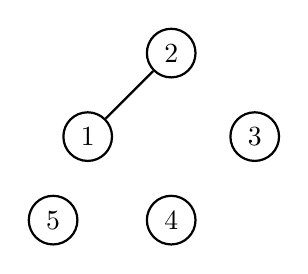
\begin{tikzpicture}[node distance={15mm}, thick, main/.style = {draw, circle}]
            \node[main] (1) {1};
            \node[main] (2) [above right of=1] {2};
            \node[main] (3) [below right of=2] {3};
            \node[main] (4) [below left of=3] {4};
            \node[main] (5) [left of=4]{5};
            \draw (1) -- (2);
        \end{tikzpicture}

    \egroup
\end{document}
